\documentclass[12pt, fullpage, a4paper]{article}
\usepackage{graphicx, latexsym}
\usepackage{setspace}
\usepackage{subfigure}
\usepackage{apacite}
\usepackage{amssymb, amsmath, amsthm}
\usepackage{bm}
\usepackage{epstopdf}
\usepackage{rotating} %used for \sidewaystable
\usepackage{apacite}
\usepackage{booktabs} %used for \toprule
\usepackage{multirow} %used for \multirow and \multicolumn
\usepackage{pifont}
\usepackage{listings}
\usepackage[svgnames]{xcolor}
%\singlespacing
%\onehalfspacing
\doublespacing
\lstset{language=R,
	basicstyle=\small\ttfamily,
	stringstyle=\color{DarkGreen},
	otherkeywords={0,1,2,3,4,5,6,7,8,9},
	morekeywords={TRUE,FALSE},
	deletekeywords={data,frame,length,as,character},
	keywordstyle=\color{blue},
	commentstyle=\color{DarkGreen},
}


\begin{document}
\title{Graphical and numerical diagnostic tools to assess multiple imputation models by posterior predictive checking}
\date{}
\maketitle
\section{Introduction}
Multiple imputation (MI) is a popular approach for the analysis of incomplete datasets. It involves generating several plausible imputed datasets and aggregating different results into a single inference. Missing cells are filled with synthetic data drawn from corresponding posterior predictive distributions. This procedure is repeated multiple times, resulting in several imputed datasets. The scientific interests are then estimated for each imputed dataset by complete-data analyses. Finally, different estimates are pooled into one inference using Rubin's rule, which accounts for within and across imputation uncertainty \cite{RubinD1987}. 

A crucial part of the multiple imputation process is selecting sensible models to generate plausible values for the missing data. The validity of post-imputation analyses relies on the compatibility of the imputation model and the substantive model of interest (Bartlett et al., 2015)\nocite{bartlett2015multiple}. This is, however, not a trivial model selection process in real life since there are usually a wide array of candidate models to check. Researchers should consider which variables, interaction terms, and nonlinear terms are included based on the scientific interest and the data features.  

Despite the popularity of multiple imputation, there are only a few imputation model diagnostic methodologies. One common diagnostic method is to compare distributions of the observed data and the imputed data (Van Buuren, 2018;\nocite{Buuren2018} Abayomi et al., 2008\nocite{abayomi2008diagnostics}). Plausible imputation models would generate imputed values that have a similar distribution to the observed data. Although missing at random (MAR) mechanisms would also induce the discrepancies between the observed and imputed data, any dramatic departures that cannot be explained by the observed data features are evidence of potential imputation model misspecification. Reliable interpretation of the observed and imputed data's discrepancies could be derived from external knowledge about the incomplete variables and the missingness mechanisms (Abayomi et al., 2008). 

The idea to evaluate the validity of scientific models on multiply imputed data is not new. Bondarenko and Raghunathan (2016)\nocite{bondarenko2016graphical} proposed an advanced diagnostic method to compare the distributions of the observed and imputed data conditional on the probability of missingness. Gelman et al. (1998)\nocite{gelman1998not} applied cross-validation to check the fit of a hierarchical Bayesian model in the study of 51 public opinion polls preceding the 1988 U.S. Presidential election. Gelman et al. (2005) also proposed to apply graphical posterior predictive inference on the test statistics for model checking with missing and latent data. If regression-based imputation approaches are involved, the conventional regression diagnostics, such as plots of residuals and outliers, are useful (White et al., 2011)\nocite{white2011multiple}. A comprehensive overview of model diagnostic in multiple imputation is available in Nguyen et al. (2017)\nocite{nguyen2017model}.

Posterior predictive checking (PPC) has been proposed as an alternative method for the imputation model diagnostic (Gelman et al., 2005; He and Zaslavsky, 2012; Nguyen et al., 2015\nocite{nguyen2015posterior}). PPC is a Bayesian model checking approach that compares the replicated data drawn from the corresponding posterior predictive distribution to the observed data. If the model lacks fit, there could be a discrepancy between the replicated data and the observed data. 

He \& Zaslavsky (2012) and Nguyen et al. (2015) applied posterior predictive checking to assess the inadequacies of the joint imputation model with one or more test quantities relative to the scientific interest. To evaluate the `usability' of imputation model with respect to the test statistics, analysts compares the estimates for the complete data and their replicates, $Q(Y_{obs}, Y_{mis} - Q(Y^{rep}_{com}))$. Comparisons of the complete data and its replicates ensure the calculation of test quantities with general missingness patterns. However, it also results in sensitivity to the amount of missingness.    

In this manuscript, we propose and evaluate an implementation of posterior predictive checking for imputation techniques that rely on the observed data. The general idea is that if the imputation model is compatible with the substantive model, the observed data is expected to locate in the center of corresponding predictive posterior distributions. We compare the completed data and their posterior replicates simulated under the model and evaluate the location of the observed data. This distinguishes our approach from the posterior predictive checking of imputation models by applying target analyses. We demonstrate:
\begin{enumerate}
	\item that PPC can be generalized to variable-by-variable imputation techniques; 
	\item that PPC can be used to identify the imputation model that conforms most to the true data generating model;
	\item that PPC can be used as a model evaluation technique to identify the better substantive analysis model;
	\item PPC with \texttt{MICE} on a real-life data set;
	\item this PPC approach is not sensitive to the amount of missing data.
\end{enumerate}
The remainder of this manuscript is organized as follows. In section 2, we review the posterior predictive checking of the imputation model by applying target analysis proposed by He \& Zaslavsky (2012). In section 3, we provide an overview of the \texttt{MICE} package and the underlying imputation algorithm: fully conditional specification (FCS). We also further point out the necessity of extending the posterior predictive checking of the imputation model so that the diagnostics would suit the \texttt{MICE} algorithm better. In section 4, we evaluate the performance of the proposed diagnostic approach with simulation studies. In section 5, we show the results of simulation studies. In section 6, we apply the proposed diagnostic approach to the body mass index (BMI) data in Dutch. In section 7, we conclude with a discussion of our findings.  

\section{Posterior predictive checking (PPC)}
With fully observed data, PPC compares the observed data with the replicated data $y^{rep}$ which are simulated from the posterior predictive distribution:
\begin{equation}
\begin{array}{ll}
p(y^{rep}|y) = \int p(y^{rep}|\theta)p(\theta|y)d\theta
\end{array} 
\end{equation}
To detect the discrepancy between the model and the data, we define test quantities which reflect the scientific interest and estimate them for both observed data and replicated data. Misfit of the model with respect to the data could be summarized by the posterior predictive p-value, which is the probability that the replicated data are more extreme than the observed data, with respect to the selected test quantities \cite{gelman2013bayesian}:
\begin{equation}
\begin{array}{ll}
p_{B} &= Pr(T(y^{rep}, \theta) \ge T(y, \theta)|y)\\
&= \int\int I_{T(y^{rep}, \theta) \ge T(y, \theta)}p(y^{rep}|\theta)p(\theta|y)dy^{rep}d\theta,
\end{array} 
\end{equation}
where $I$ is the indicator function. An extreme p-value (close to 0 or 1) implies the suspicion on the fit of the model since a consistent discrepancy between test quantities $T(y^{rep}, \theta)$ and $T(y, \theta)$ cannot explained by simulation variance. 

Posterior predictive checking has been widely used for model diagnostic in applied Bayesian analysis (Gelman et al., 2013, chapter 6) and the posterior predictive distribution is usually calculated by simulation. Suppose we have $N$ draws of model parameters from its posterior distribution $\theta_j, j=1,\dots,N$, we then generate a replicated data for every theta $\theta_j$. The PPC compares test quantities based on observed data with the empirical predictive distribution of test quantities. The estimated posterior predictive p-value is the proportion of these N simulations for which $T_{j}(y^{rep}, \theta) > T_{j}(y, \theta)$. It is noticeable that PPC's application for the imputation model diagnostic is not based on the hypothesis test perspective. Hence there is no underlying assumed distribution for the posterior predictive p-value in this case. The posterior predictive p-value indicates whether the model would provide plausible inference based on the data with respect to the selected test quantities. 

To perform multiple imputation model check with PPC, we compare the completed data, the combination of the observed and imputed data, with its replications. Gelman et al. (2005) applied graphical PPC to visualize test quantities comparisons based on completed data and the replicated data. He \& Zaslavsky (2012), and Nguyen et al. (2015) developed numerical posterior predictive checks as target analyses to the joint imputation model. He and Zaslavsky (2015) proposed two kinds of discrepancies, completed data discrepancy and expected completed-data discrepancy, and the approaches to calculate corresponding posterior predictive p-values. We briefly introduced these discrepancies and p-values for the completeness of PPC for MI models.

\subsubsection{Complete data discrepancy}
To assess the complete data discrepancy $T(y_{com}^{rep}, \theta) - T(y_{com}, \theta)$, we draw imputed values for $y_{mis}$ and $y_{com}^{rep}$ from their posterior predictive distribution:
\begin{equation}
\begin{array}{ll}
p(y_{com}^{rep}, y_{mis}|y_{obs}) = \int p(y_{com}^{rep}|\theta)p(y_{mis}|y_{obs}, \theta)p(\theta|y_{obs})d\theta
\end{array} 
\end{equation}
To assess the model fit, we calculate the posterior predictive p value as :
\begin{equation}
\begin{array}{ll}
p_{B, com} &= Pr(T(y_{com}^{rep}) \ge T(y_{com})|y_{obs})\\
&= \int\int I_{T(y_{com}^{rep}) \ge T(y_{com})}p(y_{com}^{rep}, y_{mis}|y_{obs})dy_{com}^{rep}dy_{mis}
\end{array} 
\end{equation}
The simulation process to estimate p-value proposed by He and Zaslavsky (2012) is:
\begin{enumerate}
	\item Simulate $N$ draws of $\theta$ from the corresponding posterior distribution $p(\theta|y_{obs})$
	\item For each $\theta_{j}, j=1, \dots, N$, impute $y_{mis}^j$ from $p(y_{mis}|y_{obs}, \theta_{j})$ and simulate the replicated data $y_{com}^{rep, j}$ from $p(y_{com}^{rep}|\theta_{j})$
\end{enumerate}
A $p_{B, com}$, which is close to 0 or 1, implies the discrepancy between the model and the data with respect to the selected test quantities.  
\subsubsection{Expected complete data discrepancy}
He and Zaslavsky (2012) noticed that the power of complete data discrepancy is weakened because the variance of imputed data across complete data $y_{imp}$ and replicated data $y_{imp}^{rep}$ increase the variance of the test quantities. He and Zaslavsky (2012) reduced the variance of complete data discrepancy by calculating the expectation value of missing data for each model parameter draw. 
The modification of p-value $p_{B, ecom}$ would be:  
\begin{equation}
\begin{array}{ll}
p_{B, ecom} &= Pr(E[T(y_{com}^{rep})|y_{obs}^{rep}, y_{obs}] \ge E[T(y_{com})|y_{obs}^{rep}, y_{obs}]|y_{obs})\\
&= \int\int I_{E[T(y_{com}^{rep})|y_{obs}^{rep}, y_{obs}] \ge E[T(y_{com})|y_{obs}^{rep}, y_{obs}]}p(y_{obs}^{rep}, y_{obs})dy_{obs}^{rep}
\end{array} 
\end{equation}
Again, the nested simulation process to calcualate the p-value $p_{B, ecom}$ is:
\begin{enumerate}
	\item Simulate $N_{1}$ draws of $\theta$ from the corresponding posterior distribution $p(\theta|y_{obs})$
	\item For each $\theta_{j}, j=1, \dots, N_{1}$, impute $y_{mis}^j$ from $p(y_{mis}|y_{obs}, \theta_{j})$ and simulate the replicated data $y_{com}^{rep, j}$ from $p(y_{com}^{rep}|\theta_{j})$
	\item For each j-th replicate, calculate the mean discrepancy by setting $y_{mis}^j$ and $y_{com}^{rep, j}$ to missing and overimputing them with the same paramters $\theta_{j}$ over $N_{2}$ draws $y_{mis}^{j, k}$ and $y_{com}^{rep, j, k}, k = 1, \dots, N_{2}$. Calculate the difference : $D_{j, k} = T(y_{obs}^{rep, j}, y_{mis}^{rep, j, k}) - T(y_{obs}, y_{mis}^{rep, j, k})$ over $N_{2}$ draws and then average the difference for the j-th replicate : $\bar{D}_{j.} = \sum_{1}^{k}D_{j, k}/k$
	\item Calculate $p_{B, ecom}$ as the proportion of these $N_{1}$ estimates that are positive, $\bar{D}_{j.} \ge 0$    
\end{enumerate}

He and Zaslavsky (2012) evaluated whether the PPC could detect the uncongeniality of the imputation model. Nguyen et al. (2015) investigated the performance of PPC in other imputation model misspecification scenarios such as ignoring the response variable and auxiliary variables or failing to transform skewed variables. The PPC approach proposed by He and Zaslavsky (2012) is based on the joint imputation model. The imputation model for diagnostic is a joint distribution for the observed data, and the test quantities depend on multiple variables and parameters. 
 
\section{\texttt{MICE} package}
There are two popular approaches for multiple imputation: joint modeling(JM) and fully conditional specification (FCS). JM involves specifying a multivariate distribution for the missing data and generate imputations from the conditional distribution based on different missing patterns. For example, suppose that for an incomplete dataset $Y = (Y_1, Y_2, Y_3, Y_4)$ the missing pattern for case $i$ is $r_{[i]} = (0, 0, 1, 1)$, where 0 denotes missing and 1 denotes being observed, JM specifies a joint modeling for these four variables and impute the case $i$ with the bivariate conditional distribution $P_{i}(Y_1^{mis}, Y_2^{mis} | Y_3^{obs}, Y_4^{obs}, \theta_{1,2})$. 

FCS attempts to specify an imputation model for each missing variable $Y_j$ conditional on all the other variables $P(Y_j | Y_{-j}, \theta_{j})$. It generates imputations iteratively over all missing variables after an initial imputation, such as mean imputation or random draw from observed values. Given the most recent imputations of the other missing variables $Y_{j}^{t}$ at iteration $t$, the algorithm of generating imputations for the missing variable $Y_{j}$ consists of the following draws:
\begin{align*}
\theta_{j}^{t} \sim f(\theta_{j})f(Y_{j}^{obs}|Y_{-j}^{t-1}, \theta_{j})\\
Y_{j}^{mis(t)} \sim f(Y_{j}^{mis}|Y_{-j}^{t}, \theta_{j}^{t}),
\end{align*}
where $f(\theta_{j})$ is the prior distribution for the parameter of the imputation model $\theta_{j}$.
The FCS is an attractive imputation approach because of its flexibility in imputation model specification. It is known under different names: chained equations stochastic relaxation, variable-by-variable imputation, switching regression, sequential regressions, ordered pseudo-Gibbs sampler, partially incompatible MCMC, and iterated univariate imputation \cite{van2007multiple}. 

Multivariate Imputation by Chained Equations (\texttt{MICE}) is the name of software for imputing incomplete multivariate data by Fully Conditional Specification (FCS). It has developed into the de facto standard for imputation in \texttt{R} and is increasingly being adopted in Python (e.g. statsmodels (imputer function) \& miceforest). The \texttt{MICE} package creates functions for three components of FCS: imputation, analysis, and pooling. 
\begin{figure}[ht!]
	\centering
	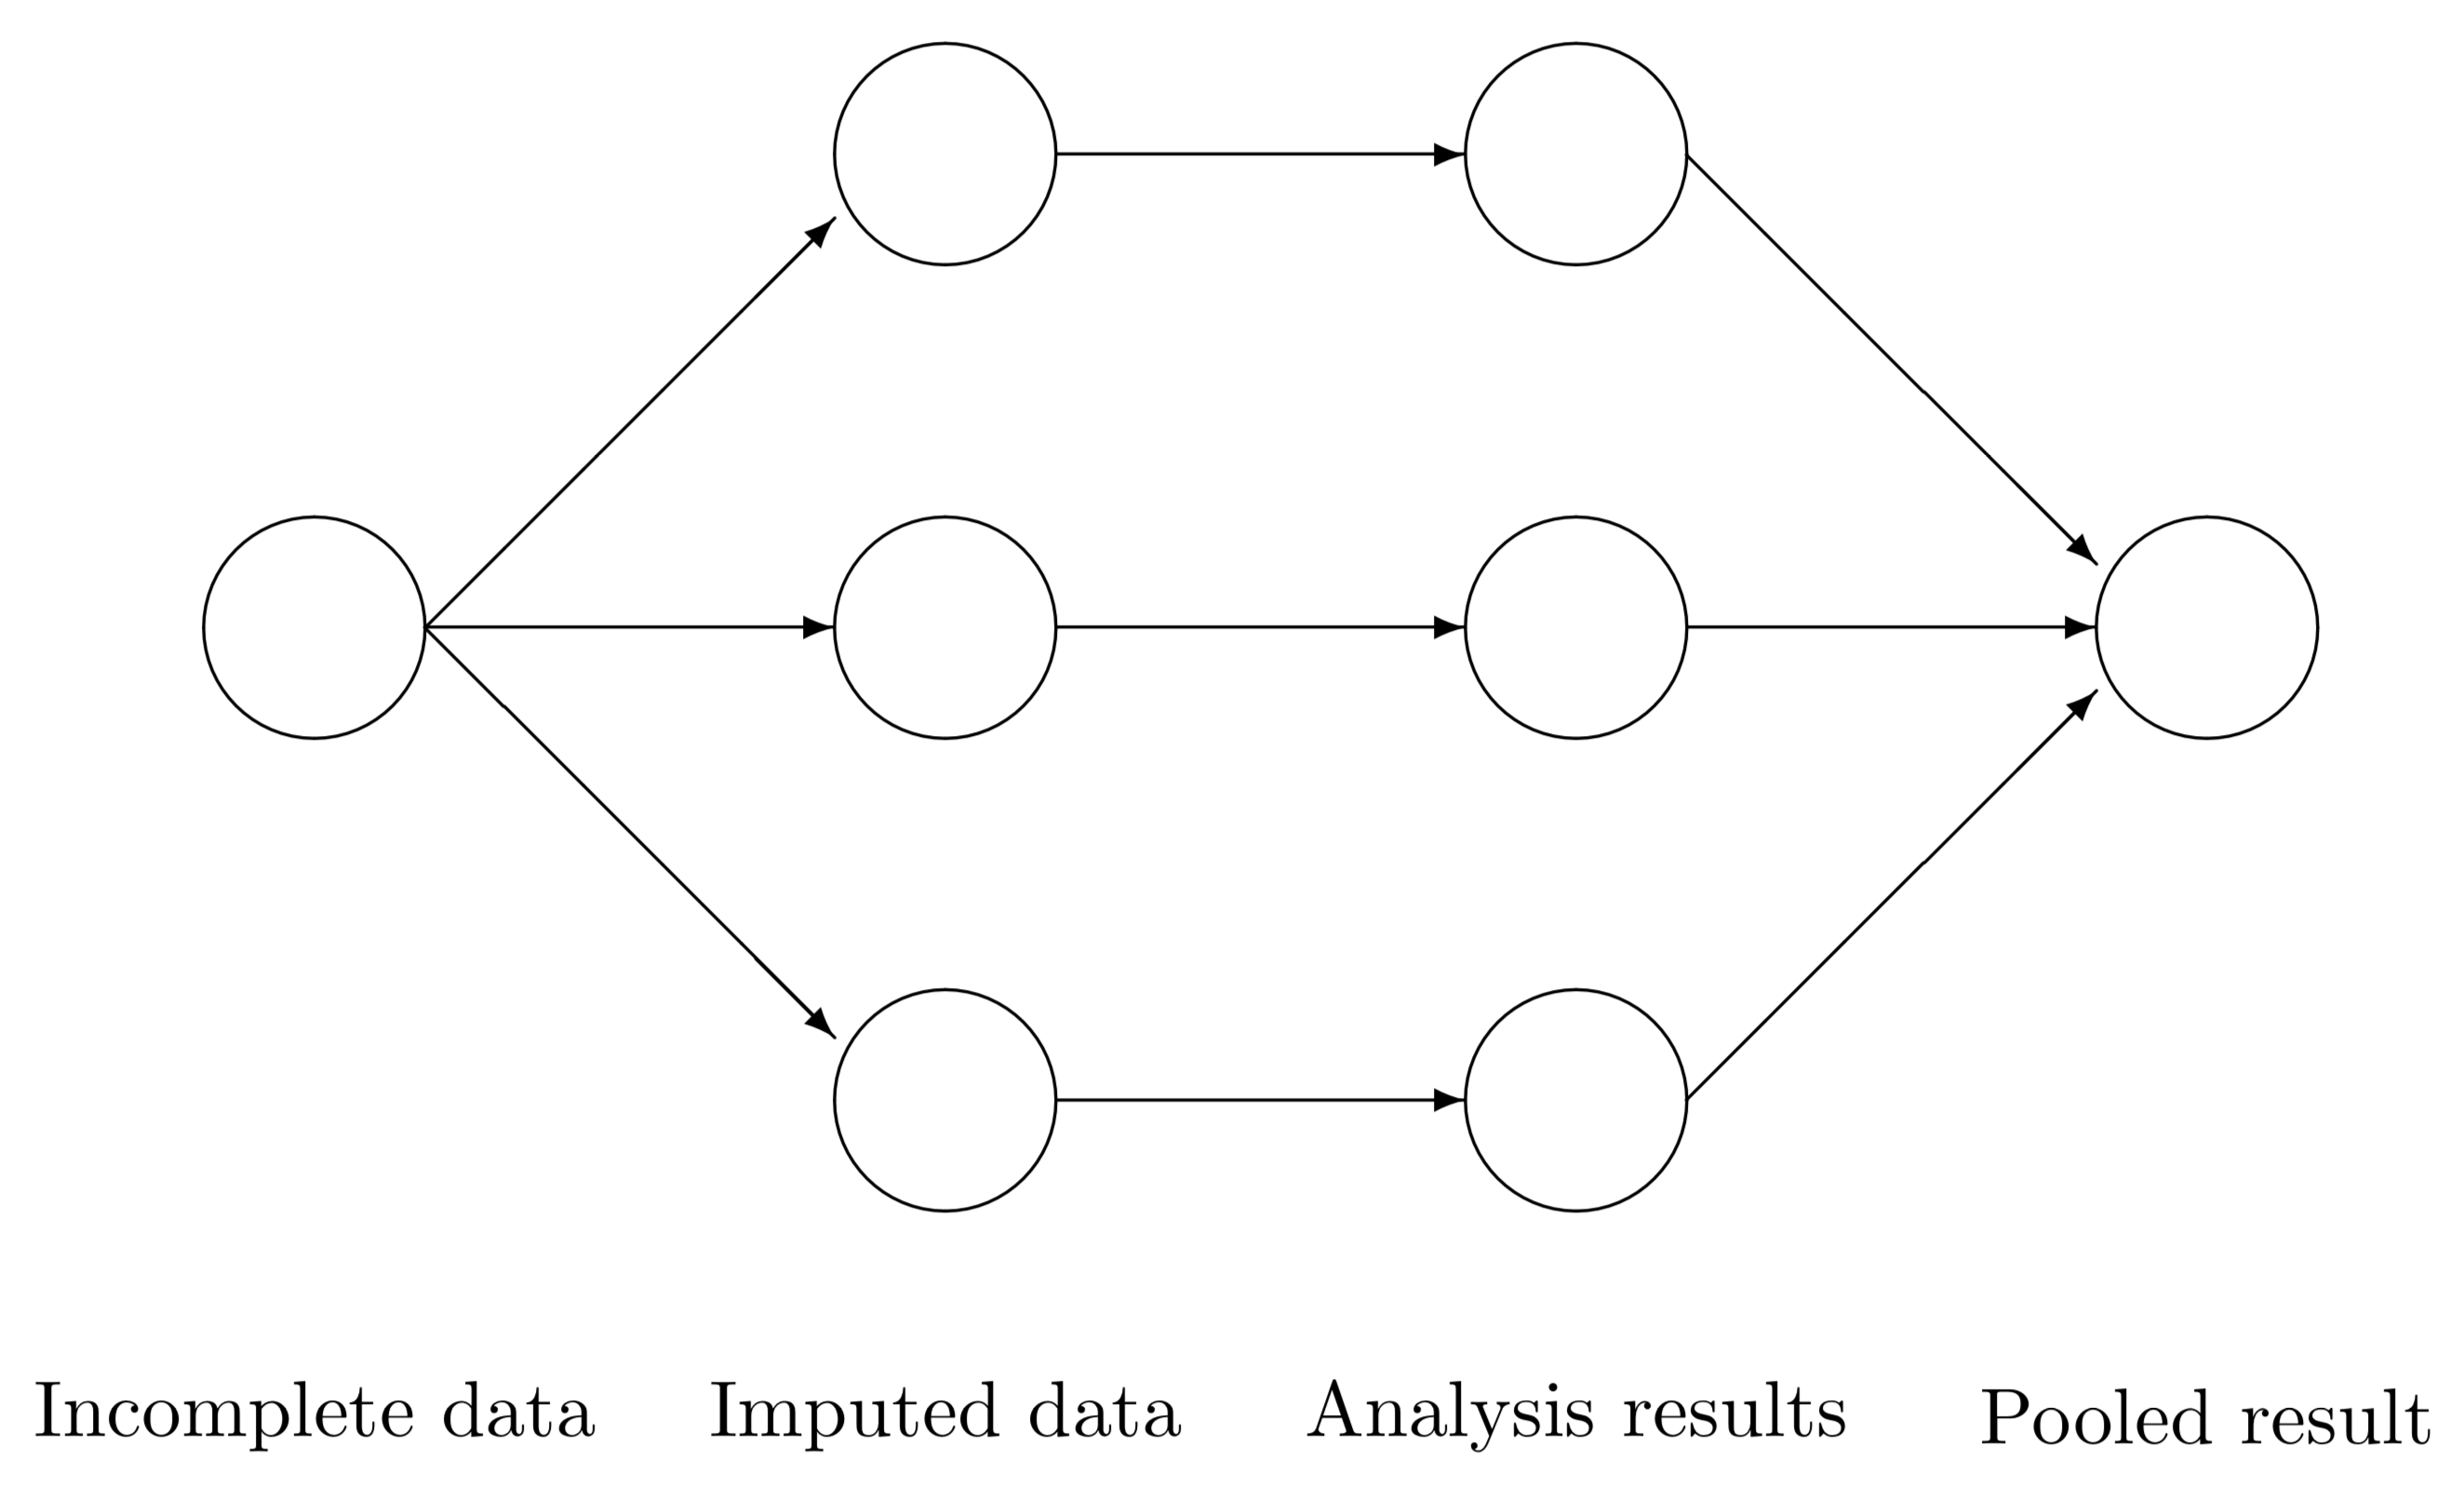
\includegraphics[scale=.2]{plot/miflow}
	\caption{Main steps used in \texttt{MICE} (van Buuren \& Groothuis-Oudshoorn, 2010)}
	\label{fig1}
\end{figure} 
Figure \ref{fig1} illustrates how MICE solves a missing data problem by generating 3 imputed datasets. Three imputed datasets are generated with function \texttt{mice()}. Analysis are performed on every imputed dataset by \texttt{with()} function and combined into a single inference with function \texttt{pool()}. The software stores the output of each step in a particular class: \texttt{mids}, \texttt{mira} and \texttt{mipo}. More details aboout \texttt{MICE} package can be found in van Buuren \& Groothuis-Oudshoorn (2010).\nocite{buuren2010mice}

Two features of the software motivate our research. First, the default imputation method for numerical missing data is predictive mean matching (PMM).
\begin{lstlisting}
library(mice, warn.conflicts = FALSE)
imp <- mice(nhanes, print = FALSE)
imp$method
\end{lstlisting}
\begin{verbatim}
##   age   bmi   hyp   chl 
##    "" "pmm" "pmm" "pmm"
\end{verbatim}
It generates imputations for a missing cell from its p nearest points. The distance function applied to selection nearest points in MICE is:
\begin{equation}
\begin{array}{ll}
d_{mice}(x_{i}^{obs}, x_{j}^{mis}) = |x_{i}^{obs}\beta^{*} - x_{j}^{mis}\hat{\beta}|,
\end{array} 
\end{equation}
where $\hat{\beta}$ is the mean of posterior distribution of models' parameters and $\beta^{*}$ is a random draw from the corresponding posterior distribution. Predictive mean matching is a nonparametric imputation approach which is proven to perform well in a wide range of scenarios (De Waal et al., 2011;\nocite{de2011handbook} Siddique and Belin, 2007;\nocite{siddique2008multiple} Su et al., 2011;\nocite{su2011multiple} Van Buuren, 2018; Van Buuren and Groothuis-Oudshoorn, 2010; Vink et al., 2014;\nocite{vink2014predictive} Vink et al., 2015;\nocite{vink2015partioned} White et al., 2011; Yu, Burton and Rivero-Arias, 2007\nocite{yu2007evaluation}). The attractive advantage of PMM is that the imputed data is consistently within the range of the sample space. (Heeringa et al., 2001;\nocite{heeringa2001multivariate} Van Buuren, 2018; Vink et al., 2014; Vink et al., 2015; White et al., 2011; Yu et al., 2007) For instance, PMM prevents imputing negative values for data that are strictly non-negative. Second, \texttt{mids} only stores imputed datasets not the estimated parameters of the imputation models. 

Based on the features of \texttt{MICE} package discussed above, it is necessary to investigate whether PPC could check the donor selection procedure of PMM and perform PPC based on the observed data itself instead of the target statistics. He and Zaslavsky (2012) briefly discussed the approach to checking imputation models for subsets of missing variables. However, they assumed that the imputations of remaining variables (excluding the incomplete variables of interest in an assessment) are adequate. We also evaluate the performance of PPC when relaxing this assumption in the application section.      

The implement of PPC for multiple imputation models in \texttt{MICE} package is straightforward. Suppose we would like to diagnose the compatibility of the imputation model for a block of missing variables $Y_{interest}$, we duplicate the complete cases of $Y_{interest, obs}$ and remove the values of $Y_{interest}$ in the duplication part $Y^{dup, mis}_{interest, obs}$. It is noticeable that we discard the cases with missing cells in $Y_{interest}$ in the original dataset. The derived concatenated dataset has two parts of the same cases. One half is the cases with completely observed $Y_{interest}$ in both original data and the concatenated data. The other half is the cases with completely observed $Y_{interest}$ in original data but removed the observed value deliberately in the concatenated data. The remaining variables could also be partially observed. To perform the PPC for the imputation model of $Y_{interest}$, we apply \texttt{mice} function in \texttt{MICE} package to impute the concatenated data. Imputation values for $Y^{dup, mis}_{interest, obs}$ in a number of iterations forms the posterior distribution for each case with completely observed $Y_{interest}$. To derive stable posterior distribution, the number of iterations $nit$ should not be too small. He and Zaslasky (2012) suggested it is sufficient to set $nit$ from 20 to 50..     

\section{Simulation Study}
We carry out a simulation study to illustrate the performance of the proposed diagnostic approach, varying several factors including missingness proportion (30\%, 50\%, 80\%), missingness mechanisms (MCAR and MARr), nominal levels of the confidence interval (75\%, 95\%) and different imputation models. The simulation study consists of diagnostics under three different scenarios: 1) linear regression model with squared terms with a missing outcome 2) linear regression model with squared terms with a missing covariate and the corresponding quadratic term 3) generalized linear model with a missing binary outcome. We evaluate whether the proposed diagnostic method could identify the compatible imputation model for continuous and discrete missing variables under the first and the third scenarios. We also investigate the performance of the proposed diagnostic method on the donor selection procedure of predictive mean matching under the second scenario. The sample size and the number of iterations are set to be 1000 and 50 separately in all simulations.  

We induce missingness with \texttt{ampute()} function in the simulation study. Generally, \texttt{Ampute()} is a convenient function in \texttt{MICE} package to generate missing data for simulation purposes (Schouten et al. 2017)\nocite{Schouten2018}. We consider missing completely at random (MCAR) mechanisms where the probability of missing is equal for every cell and right-tailed missing at random (MARr) mechanisms where higher values of covariates have a higher probability of being unobserved. In the algorithm of \texttt{ampute()} function, the probability of missing is allocated with different logistic functions of weighted sum scores, which is a linear combination of covariates correlated with the probability of missing:
\begin{equation}
\begin{array}{ll}
wss_{i} = w_{i}x_{1i} + w_{i}x_{2i} + \dots + w_{i}x_{mi}
\end{array} 
\end{equation}
The weight $w_i$ is pre-specified to reflect the influence of the variable $x_{i}$ on the probability of missing. For instance, if the formation of a weighted sum score is:
$wss = x_1 + x_2$, the probability of missing is determined by both $x_1$ and $x_2$ with the equal effects. More specifically, under MARr mechanisms, candidates with higher values of weighted sum scores have a higher probability of being unobserved when applying \texttt{ampute()} function to generate missing data.

\subsection{linear regression model for continuous variables}
We consider a partially observed variable $Y$ and a fully observed variable $X$. The data is generated from : $X \sim unif(-3, 3)$, $Y|X \sim \mathcal{N}(X + X^2, 1)$. The scientific model is indeed a quadratic model. We consider two imputation models for the missing response $Y$: one is a linear regression of $Y$ on $X$, and the other one is a quadratic regression of $Y$ on $X$. 

\subsection{Quadratic term regression}
The response variable $Y$ is generated from a normal distribution : $Y|X \sim \mathcal{N}(X + X^2, 1)$, where the covariate $X$ follows a standard normal distribution. In this simulation study, the response variable $Y$ is completely observed while the covariate $X$ and the corresponding quadratic term $X^2$ are jointly missing for a part of cases. There are no cases with missing cells on either $X$ or $X^2$. We compare two non-parametric methods, predictive mean matching (PMM) and polynomial combination (PC) with a parametric method, the substantive model compatible fully conditional specification (SMC-FCS). The PC and SMC-FCS methods are two accepted methods to impute linear regression with quadratic terms. The PC method is an extension of PMM but applies a different donors selection procedure. 

\subsection{Generalized linear model for discrete variables}
We consider a partially observed binary $Y$ and two complete covariates $X$ and $Z$. The model of scientific interest is : $Pr (Y = 1 | X, Z) = exp(X + Z) / 1 + exp(X + Z)$,
where $x \sim unif(-3 , 3)$ and $Z \sim \mathcal{N}(1, 1)$. Under MARr mechanism, the weights of variables $X$ and $Z$ in the determining of the probability of missing for $Y$ are set to be equal. Since the logistic regression actually model the probability of assignment, we investigate the plot of deviance and calculate the sum of squared deviance divided by the sample size. There are two candidate models: a logistic regression of $Y$ on $X$ and $Z$ and a logistic regression of $Y$ on $Z$ only.

\section{Simulation results}
In this section, we present the simulation results of the proposed diagnostic method under three different scenarios. For numerical assessment, We estimate the rate of nominal confidence interval covers the observed data (COV), the mean of the distance between the observed data and the location of the predictive posterior distribution (Distance), and the average width of the nominal confidence intervals (CIW). We also provide graphical analysis with scatterplot, density plot and distribution plot, which shows the means and nominal confidence intervals for each observed data.  

\subsection{linear regression model for continuous variables}
Table \ref{tab1} shows the rate of nominal confidence interval covers the observed data, the mean of the distance between the observed data and the location of the predictive posterior distribution, and the average width of the nominal confidence intervals. Since we only generate one incomplete dataset and repeat imputing it 50 times, all coverage rates are close to the pre-specified nominal level. However, when the imputation model is misspecified as a linear regression model, the average distance is larger than the average distance under the correct specification of the imputation model (linear regression with a quadratic term). It proves our intuitive idea that the data would be close to the center of predictive posterior distributions if the model fits. The variance of the missing variable $Y$ is set as 1, which implied that the width of 95\% nominal confidence interval is approximate 3.92 (1.96 * 2) and the width of 75\% nominal confidence interval is approximate 2.3 *(1.15 * 2). When the imputation model is correctly specified, the estimated average width of the confidence interval is unbiased. However, the variance of $Y$ is overestimated when the imputation model is linear. 

The same result could also be derived from the graphical analysis. Figure \ref{fig2} shows means and 95\% confidence intervals (distribution plot) under the scenario of 30\% missing cases and MARr missing mechanism. When the imputation model is correctly specified, the points out of the 95\% confidence interval randomly spread over the sample space without any patterns. However, when the imputation is incorrectly specified as the linear regression model, the points out of the confidence interval cluster in the regions with extreme values of $X$. The density plot and the scatter plot of the observed and replicated data generated with function \texttt{densityplot()} and \texttt{xyplot()} in \texttt{MICE} also shows the evidence that the quadratic regression is preferable than the linear model (see figure \ref{fig3}). The scatter plot of the quadratic regression imputation model shows that replicated data overlap the observed data. The density plot shows the replicated data shares the same distribution with the observed data. This evidence illustrates the compatibility of the quadratic regression imputation model. While the linear regression model performs worse than the quadratic regression model: first, the replicated data do not cover the observed data in two extreme regions in the scatter plot. Second, the empirical density of the replicated data and observed data are different. However, these three plots do not merely illustrate the misspecification of the imputation model as the linear regression model. It also provides information to identify the regions of sample space in which the sub-optimal imputation model could still generate acceptable imputed values. Based on the plot of means and 95\% confidence intervals for the linear regression imputation model, we could also develop the piecewise linear regression model for the observed data. 

When we cannot figure out the imputation model under which the observed data fit the predictive posterior distribution perfectly, these plots based on observed data provide the evidence of rebuild a contamination imputation model, which would improve the validity of imputation values. When the missing cases are not in the regions where outliers crowd, we could even apply the incompatible imputation model. For example, in our simulation scenarios, suppose we only consider the linear regression imputation model and missing cases with near the parabolic minimum $X$ values, the imputed value will not show larger deviations from the true value. Finally, our proposed PPC approach for imputation model is robust against different percentage of missing cases, missingness mechanisms, and the confidence interval's nominal levels. The nominal level of the confidence interval is determined with the extent to which we could undertake the outliers when the imputation model is not compatible with the data generating process. For instance, there are more outliers in the plot of means and 75\% confidence intervals than the plot of mean and 95\% confidence intervals. When we would like to replace the linear regression model with a piecewise linear model to improve the imputation, the selection knots based on the 75\% confidence intervals are more closed to the parabolic minimum than the 95\% confidence intervals (See figure \ref{fig4}). 

\subsection{Quadratic term regression}
Table \ref{tab2} and \ref{tab3} show the result of simulations, including the coverage rate of the nominal confidence interval, the mean distance between the observed data and the center of the predictive posterior distribution and the average width of the nominal confidence interval. Based on the numerical result, the performance of these three methods, PC, SMC-FCS, and PMM, is the same, despite the slightly reduced coverage rate of PMM. In fact, when the missingness mechanism is MCAR (to bypass the problem of the sparse observed region for PMM), the PMM would also provide the valid inference of the regression weights (see Table \ref{tab4}).

However, when it comes to the graphical diagnostics, the misfit of PMM appears. The distribution plot (figure \ref{fig7} and \ref{fig8}) show that PC and SMC-FCS generate the same posterior predictive distribution of the observed data. There are more outliers with a larger value of $Y$. It is sensible since the density function of $X$ based on $Y$ is not monotone, it is unavoidable to impute the missing cell on the opposite arm of the parabolic function. Although in such a case, the imputed value is not the same as the true value, the replicated data still overlap the observed data in the scatter plot and shares the same empirical posterior distribution with the observed data (see Figures \ref{fig5} and \ref{fig6} ). The plot of mean and 95\% nominal confidence interval of PMM in Figure \ref{fig7} does not show more outliers than these of PC and SMF-FCS. However, when the nominal level is set as 75\%, more outliers appear in the sub-plot of PMM (Figure \ref{fig8}). The reason is that there more observed data closed to the center in the plots of PC and SMC-FCS, which implies the preferable of PC and SMC-FCS. The scatter plot and density plot also show the discrepancy between the distribution of the replicated and the observed data with respect to PMM (Figures \ref{fig5} and \ref{fig6}). The result is robust against various percentages of missing cases and missing mechanisms. The proposed PPC for imputation model could check the donors selection process of hot-deck approaches. In our simulation scenarios, selecting donors for the composed variable $X + X^2$ is better than for the missing variable $X$ only. The SMC-FCS is treated as the baseline in our simulation since it is proven as a reliable imputation method when the substantive model is known (Bartlett et al., 2015). The PC performs as well as the SMC-FCS which implies the donor selection process of PC reflects the data generating process in our simulation scenarios. However, when applying hot-deck approaches to implement imputation, the success in model checking is not sufficient to valid imputations. In order to determine whether we could derive plausible imputations, additional diagnoses of distributions of complete variable for observed and missing cases is necessary. For example, in our simulation scenarios, if the variable $Y$'s range of missing cases is out of the range of observed cases, the PC may still derive implausible imputations. 

\subsection{Generalized linear model for discrete variables}
The table \ref{tab5} shows the average sum of squared deviance for two different logistic regression models. The value of the average sum of squared deviance is smaller when the imputation model is correctly specified with logistic regression on both $X$ and $Z$. The result is robust against the percentage of missing cases and missingness mechanisms. Figure \ref{fig9} shows that the residuals tend to zero when the imputation model fits the observed data better. Furthermore, the peaks in the density plot (figure \ref{fig10}) also imply the empirical posterior distributions of replicated data generated under the logistic model with covariates $X$ and $Z$ are more closed to the distribution of the observed data. While the distribution of the observed data is more extreme compared with the empirical posterior distributions of replicated data generated under the logistic model with only variable $Z$. 

\section{Application}
\subsection{Background}
We illustrate the application of the proposed PPC for multiple missing variables with the data from the body mass index (BMI) of the Dutch. BMI is defined as the body weight divided by the square of the body height, which is broadly applied to categorize a person into underweight, normal, overweight, and obese. Since measuring a person's weight and height is costly, it is alternative to ask people to report their weight and height. However, such self-report data is systematically biased. People are used to overestimating their height and underestimating their weight, which leads to a lower self-report BMI compared with measured BMI. (van Buuren, 2018, section 9.3) The goal of the study is to estimate unbiased BMI from the self-report data. We apply the multiple imputation approach to fill the unobserved measured weight and height. 

The data we analyze is named \texttt{selfreport} in \texttt{MICE} package. The data consists of two components. One is the calibration dataset contains 1257 Dutch individuals with both self-report and measured height and weight which taken from Krul, Daanen, and Choi (2010)\nocite{krul2011self}. The origin survey measured 4459 adults in either Italy, Netherlands, or North America aged 18-65 years in 1999 or 2000. The second part is the survey dataset contains 803 Dutch adults aged 18-75 years with only self-reported data. The survey data were collected in November 2007, either online or using paper-and-pencil methods. (van Buuren 2018, section 9.3). Six variables are included in the application: age (years), sex(male or female), hm denoting measured height (cm), hr denoting self-reported height (cm), wm denoting measured weight (kg), and wr denoting self-reported weight (kg). 

The aim is to check whether the proposed PPC for MI works for a missing variable when imputation models for other missing variables are not appropriate. Because FCS imputed missing variables in an iteration way, the incorrect imputation model for the missing variable $Y_1$ may disturb the diagnostic for the missing variable $Y_2$. The deviation of the distribution of $Y_1$ may cause a sub-optimal imputation model becoming the optimal choice of $Y_2$. We design two linear regression imputation models for hm: one includes all the other variables; the other one includes all the other variables except the variable hr. Similarly, there are two linear regression imputation models for wm: one includes all the other variables; the other one includes all the other variables except the variable wr. In such a case, we have four imputation strategies to evaluate:
\begin{enumerate}
	\item Case 1: impute hm with linear regression model including hr and wm with linear regression including wr.
	\item Case 2: impute hm with linear regression model including hr and wm with linear regression excluding wr.
	\item Case 3: impute hm with linear regression model excluding hr and wm with linear regression including wr.
	\item Case 4: impute hm with linear regression model excluding hr and wm with linear regression excluding wr.
\end{enumerate}
Although it is obvious that hr and wr are significant covariates for the imputation of hm and wm, we deliberately ignore these two variables to reflect more discernible discrepancies for the purpose of illustration. 
\subsection{Results}
The table \ref{tab6} shows that the best imputation models among these four are the one which includes both wr and hr. The average distance and the width of confidence intervals for the observed data is the smallest for both hm and wm. No matter the imputation model of hm is correctly specified, we can conclude that the linear regression imputation model for wm should be based on all the other variables. When fixing the imputation model for the hm (no matter including hr or not), the average distance and the average width of the confidence interval of hm derived under the linear model included hr is remarkably less than the result taken under the linear model excluded the covariate hr. The graphical results (Figure \ref{fig11}-\ref{fig14}) show the same conclusion. When the linear regression imputation model for wm or hm is correctly specified, the imputed data overlap the observed data in the scatter plot. Furthermore, the observed data would be more closed to the center of the confidence interval, and the width of confidence intervals are smaller. However, the result of wr in case 3 is slightly larger than that in case 1. Similarly, the result of wr in case 4 is slightly larger than that in case 2. Two findings imply that incorrect specification of the imputation models for other missing variables $Y_j$ would influence the target variable $Y_j$ on which we perform the PPC. Our application scenario is relatively simple: the linear model is sufficient to reflect the data generating process of missing variables. However, we do not rule out the possibility that under extreme and complicated cases, incorrect specification of the imputation models for other missing variables $Y_j$ would prevent us from selecting the actual most suitable imputation model for the missing variable $Y_j$. A similar result could be found in fixing the imputation model for the wm (no matter the imputation model includes wr or not). The average distance and the average confidence interval of wm derived under the linear model had wr is remarkably less than the result taken under the linear model excluded the covariate wr.

\section{Discussion}
The proposed imputation model diagnostic procedure based on PPC works on continuous and discrete variables under parametric and hot-deck multiple imputation approaches. We could derive more information for a continuous variable, such as the blueprint of imputation model improvement, because of the graphical analysis of the predictive posterior distribution of the observed data. The imputation model selection could be determined with a numerical comparison of summarized statistics, such as the deviation between the observed value and the expectation of corresponding predictive posterior distribution or the width of confidence intervals of predictive posterior distributions for the observed data. The diagnostic could also be performed based on the graphical analysis, such as the scatter plot and the density plot of the observed and replicated data. The more suitable imputation models are, the more similar the replicated data is to the observed data in the density plot and the scatter plot. In terms of the distribution plot, the observed data would be more close to the center, and the confidence interval width is narrower. For hot-deck imputation approaches, what PPC diagnoses is the donor selection procedures. However, based on the features of predictive mean matching, the appropriate donor selection does not ensure plausible imputations. Extra analysis of the observed data and the imputed data is necessary. The PPC for categorical data or ordered data is limited since the predictor of the imputation model is the probability of assignment rather than the observed data itself. We currently investigate the residual deviance as the indicator to select the model for categorical data and ordered data. 

The applied example shows the PPC works on the multivariate missing datasets. When the imputed covariate deviates from the actual distribution because of the mis-specified imputation models, the imputation model for the predictor could also selected by PPC. In our case study, the misspecification of one missing variable slightly influences the other missing variable's numerical results. However, in more extreme situations, such as a large number of missing variables and more ridiculous imputation models for covariates, the result may be influenced seriously, so as to result in a sub-optimal model selection. It is more reasonable to perform the numerical analysis of all missing variables and make the model selection for those variables with remarkably different results under different candidate imputation approaches first. 

Existing PPC proposed by He and Zaslavsky (2012) and Gelman et al. (2015) measured the posterior predictive p-value to indicate the discrepancies of summarized statistics between the observed and replicated data. The close to 0 or 1 p-value implies the inadequacy of the imputation model with respect to the target quantities. The target quantities should be calculated with the completed data, which consists of the observed and the imputed data because it may fail to calculating the target quantities requiring a complete data matrix. Both He \& Zaslavsky (2012) and Nguyen et al. (2015) found the existing PPC for multiple imputation model is sensitive to the percentage of missing cases. Since the imputed data and the replicated data are generated from the same posterior predictive distribution, with an increasing proportion of missing data, the diagnose becomes more difficult.

Unlike the existing PPC approach, the PPC discussed in the paper check the imputation model for each missing variable under the FCS framework. We diagnose the distribution of the observed data so that the result would also be reliable with a large proportion of missing cases. The simulation study also shows the proposed PPC works for different missingness mechanisms. The PPC for multiple imputation models based on target analysis would be more informative when the imputer is also the researcher. The issue would be whether valid inference for the scientific interest could be derived from the imputed data. However, the PPC for multiple imputation models based on the observed data addresses another issue: whether the imputation model is compatible with the substantive model. The imputed data generated after the proposed PPC could be used for more general downstream analysis and for different scientific interests.

When the sample size is tremendous, it is better to choose some representative data to check the imputation model so that the scatter plot or the distribution plot would not be too crowded. A clustered procedure could be applied to gather the observed data with closed values and choose one subset in each cluster to do the model checking. Further investigation is necessary to set the rule to select observed data when the sample size is too large.

\newpage
\bibliographystyle{apacite}
\bibliography{PPC}

\newpage
\begin{sidewaystable}[ht!]
	\begin{tabular}{cc|cccc|cccc|cccc}
		\multicolumn{2}{l|}{}                             & \multicolumn{4}{c|}{COV}                                                                                           & \multicolumn{4}{c|}{Average Distance}                                                                              & \multicolumn{4}{c}{Average CIW}                                                                                   \\ \cline{3-14} 
		\multicolumn{1}{l}{}      & \multicolumn{1}{l|}{} & \multicolumn{2}{c}{linear model}                        & \multicolumn{2}{c|}{quadratic model}                     & \multicolumn{2}{c}{linear model}                        & \multicolumn{2}{c|}{quadratic model}                     & \multicolumn{2}{c}{linear model}                        & \multicolumn{2}{c}{quadratic model}                     \\ \hline
		\multicolumn{1}{l|}{}     & \multicolumn{1}{l|}{} & \multicolumn{1}{l}{75\%CI} & \multicolumn{1}{l}{95\%CI} & \multicolumn{1}{l}{75\%CI} & \multicolumn{1}{l|}{95\%CI} & \multicolumn{1}{l}{75\%CI} & \multicolumn{1}{l}{95\%CI} & \multicolumn{1}{l}{75\%CI} & \multicolumn{1}{l|}{95\%CI} & \multicolumn{1}{l}{75\%CI} & \multicolumn{1}{l}{95\%CI} & \multicolumn{1}{l}{75\%CI} & \multicolumn{1}{l}{95\%CI} \\
		\multicolumn{1}{c|}{}     & missingness           &                            &                            &                            &                             &                            &                            &                            &                             &                            &                            &                            &                            \\ \cline{2-14} 
		\multicolumn{1}{c|}{}     & 30                    & 0.76                       & 0.96                       & 0.75                       & 0.93                        & 2.41                       & 2.41                       & 0.79                       & 0.79                        & 6.64                       & 11.32                      & 2.27                       & 3.87                       \\
		\multicolumn{1}{c|}{MCAR} & 50                    & 0.72                       & 0.96                       & 0.76                       & 0.94                        & 2.44                       & 2.44                       & 0.77                       & 0.77                        & 6.61                       & 11.27                      & 2.25                       & 3.83                       \\
		\multicolumn{1}{c|}{}     & 80                    & 0.77                       & 0.95                       & 0.78                       & 0.94                        & 2.25                       & 2.25                       & 0.87                       & 0.87                        & 6.53                       & 11.13                      & 2.51                       & 4.28                       \\\hline
		\multicolumn{1}{c|}{}     & 30                    & 0.75                       & 0.95                       & 0.74                       & 0.94                        & 2.28                       & 2.28                       & 0.8                        & 0.8                         & 6.26                       & 10.66                      & 2.31                       & 3.94                       \\
		\multicolumn{1}{c|}{MARr} & 50                    & 0.76                       & 0.95                       & 0.73                       & 0.95                        & 2.21                       & 2.21                       & 0.81                       & 0.81                        & 6.3                        & 10.73                      & 2.3                        & 3.91                       \\
		\multicolumn{1}{c|}{}     & 80                    & 0.8                        & 0.96                       & 0.77                       & 0.92                        & 1.8                        & 1.8                        & 0.83                       & 0.83                        & 5.43                       & 9.25                       & 2.38                       & 4.05                      
	\end{tabular}
	\caption{The performance of two imputation models under different scenarios}
	\label{tab1}
\end{sidewaystable}

\begin{sidewaystable}[ht!]
	\begin{tabular}{cc|ccc|ccc|ccc}
		\multicolumn{2}{l}{}                    & \multicolumn{3}{c|}{COV} & \multicolumn{3}{c|}{Average distance} & \multicolumn{3}{c}{Average CIW} \\ \cline{2-11} 
		\multicolumn{1}{c|}{}     & missingness & PC    & SMC-FCS  & PMM   & PC         & SMC-FCS      & PMM       & PC       & SMC-FCS    & PMM     \\
		\multicolumn{1}{c|}{}     & 30          & 0.94  & 0.94     & 0.91  & 0.62       & 0.62         & 0.68      & 3.02     & 3.1        & 3.03    \\
		\multicolumn{1}{c|}{MCAR} & 50          & 0.94  & 0.93     & 0.9   & 0.61       & 0.61         & 0.67      & 3.03     & 3.06       & 2.97    \\
		\multicolumn{1}{c|}{}     & 80          & 0.96  & 0.94     & 0.91  & 0.61       & 0.64         & 0.65      & 3.06     & 3.14       & 3       \\ \hline
		\multicolumn{1}{c|}{}     & 30          & 0.94  & 0.94     & 0.89  & 0.59       & 0.59         & 0.64      & 2.93     & 2.84       & 2.84    \\
		\multicolumn{1}{c|}{MARr} & 50          & 0.93  & 0.94     & 0.89  & 0.57       & 0.58         & 0.62      & 2.74     & 2.7        & 2.68    \\
		\multicolumn{1}{c|}{}     & 80          & 0.93  & 0.97     & 0.93  & 0.56       & 0.56         & 0.61      & 2.61     & 2.64       & 2.69   
	\end{tabular}
	\caption{The performance of PC, SMF-FCS and PMM under different scenarios. The nominal level is 95\%}
	\label{tab2}
\end{sidewaystable}

\begin{sidewaystable}[ht!]
	\begin{tabular}{cc|ccc|ccc|ccc}
		\multicolumn{2}{l}{}                    & \multicolumn{3}{c|}{COV} & \multicolumn{3}{c|}{Average distance} & \multicolumn{3}{c}{Average CIW} \\ \cline{2-11} 
		\multicolumn{1}{c|}{}     & missingness & PC    & SMC-FCS  & PMM   & PC         & SMC-FCS      & PMM       & PC       & SMC-FCS    & PMM     \\
		\multicolumn{1}{c|}{}     & 30          & 0.76  & 0.75     & 0.7   & 0.62       & 0.62         & 0.68      & 1.77     & 1.82       & 1.78    \\
		\multicolumn{1}{c|}{MCAR} & 50          & 0.75  & 0.75     & 0.73  & 0.61       & 0.61         & 0.67      & 1.78     & 1.8        & 1.74    \\
		\multicolumn{1}{c|}{}     & 80          & 0.78  & 0.76     & 0.75  & 0.61       & 0.64         & 0.65      & 1.8      & 1.84       & 1.76    \\ \hline
		\multicolumn{1}{c|}{}     & 30          & 0.76  & 0.74     & 0.71  & 0.59       & 0.59         & 0.64      & 1.72     & 1.66       & 1.67    \\
		\multicolumn{1}{c|}{MARr} & 50          & 0.74  & 0.72     & 0.69  & 0.57       & 0.58         & 0.62      & 1.61     & 1.58       & 1.57    \\
		\multicolumn{1}{c|}{}     & 80          & 0.75  & 0.73     & 0.7   & 0.56       & 0.56         & 0.61      & 1.53     & 1.55       & 1.58   
	\end{tabular}
	\caption{The performance of PC, SMF-FCS and PMM under different scenarios. The nominal level is 75\%}
	\label{tab3}
\end{sidewaystable}

\begin{table}[ht!]
	\begin{tabular}{cccc}
		& True value & Estimates value & Coverage rate \\
		$\beta_1$ & 1          & 1.008           & 0.934         \\
		$\beta_2$ & 1          & 1               & 0.958        
	\end{tabular}
	\caption{The PMM performs under the scientific model : $Y = \alpha + X\beta_{1} + X^2\beta_{2} +\epsilon$, where $\alpha = 0$, $\beta_{1} = 1$ and $\beta_{2} = 1$. The error term and variable $X$ follow standard normal distributions. 30\% cases of $X$ and $X^2$ are designed to be jointly missing. The missingness mechanism is MCAR.}
	\label{tab4}
\end{table}

\begin{table}[ht!]
	\begin{tabular}{cc|cc}
		&             & \multicolumn{2}{c}{mean of residual deviance} \\ \cline{2-4} 
		\multicolumn{1}{c|}{}     & missingness & with x               & without x               \\
		\multicolumn{1}{c|}{}     & 30          & 0.83                 & 1.25                    \\
		\multicolumn{1}{c|}{MCAR} & 50          & 0.85                 & 1.27                    \\
		\multicolumn{1}{c|}{}     & 80          & 0.95                 & 1.3                     \\ \hline
		\multicolumn{1}{c|}{}     & 30          & 0.9                  & 1.34                    \\
		\multicolumn{1}{c|}{MARr} & 50          & 0.94                 & 1.35                    \\
		\multicolumn{1}{c|}{}     & 80          & 0.98                 & 1.28                   
	\end{tabular}
	\caption{The average sum of squared deviance}
	\label{tab5}
\end{table}

\begin{table}[ht!]
	\begin{tabular}{c|ccc|ccc}
		& \multicolumn{3}{c|}{hm}               & \multicolumn{3}{c}{wm}                \\ \cline{2-7} 
		& cov  & average distance & average CIW & cov  & average distance & average CIW \\
		strategy 1 & 0.95 & 1.57             & 8.27        & 0.95 & 2.28             & 12.46       \\
		strategy 2 & 0.95 & 1.65             & 8.89        & 0.94 & 10.9             & 54.38       \\
		strategy 3 & 0.95 & 5.58             & 26.89       & 0.94 & 2.35             & 12.83       \\
		strategy 4 & 0.95 & 5.56             & 27.88       & 0.97 & 9.84             & 59.57      
	\end{tabular}
	\caption{The performance of 4 imputation strategies summarized by the coverage rate, the average distance and the average width of confidence intervals with respect to missing variables hm and wm}
	\label{tab6}
\end{table}

\newpage
\begin{figure}[b]
	\begin{center}
		\resizebox{\textwidth}{!}{
			\subfigure[quadratic imputation model]{
				\label{boxplot:a}
				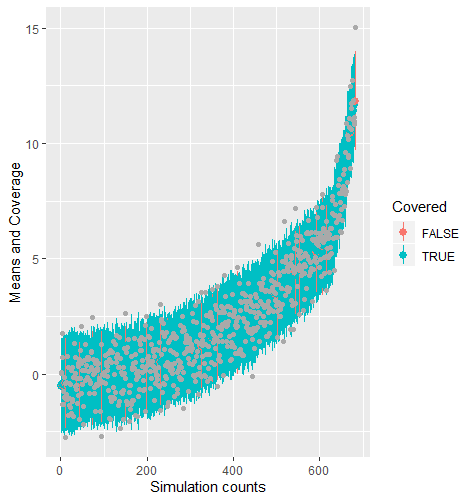
\includegraphics[scale=.5]{plot/1}
			}
			\subfigure[linear imputation model]{
				\label{boxplot:b}
				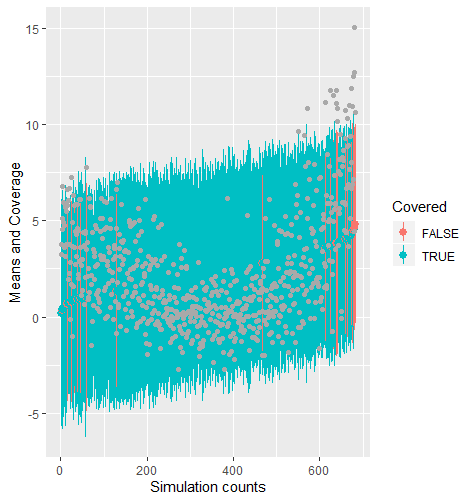
\includegraphics[scale=.5]{plot/2}
			}
		}
	\end{center}
	\caption{Distribution plots are generated under 30\% missing cases and MARr missingness mechanism. The confidence interval is 95\% nominal.}
	\label{fig2}
\end{figure}

\begin{figure}[t]
	\begin{center}
		\resizebox{\textwidth}{!}{
			\subfigure[quadratic imputation model]{
				\label{boxplot:a}
				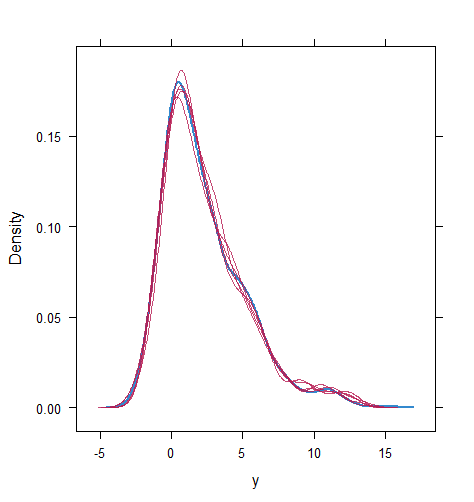
\includegraphics[scale=.5]{plot/3}
			}
			\subfigure[linear imputation model]{
				\label{boxplot:b}
				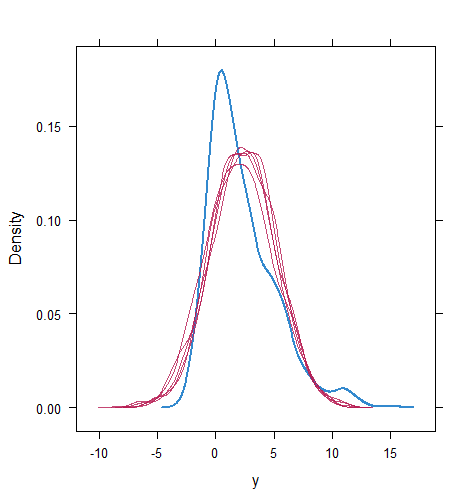
\includegraphics[scale=.5]{plot/4}
			}
		}\\ 	
		\resizebox{\textwidth}{!}{
			\subfigure[quadratic imputation model]{
				\label{boxplot:c}
				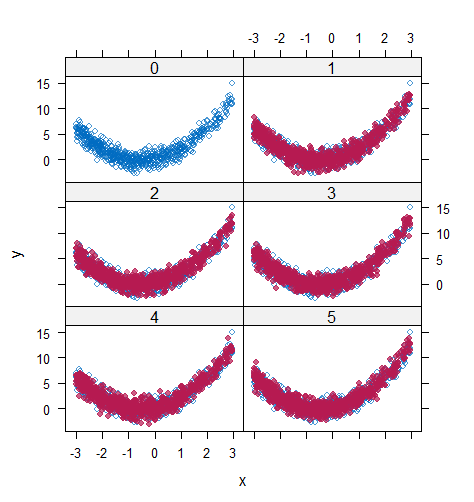
\includegraphics[scale=.5]{plot/5}
			}
			\subfigure[linear imputation model]{
				\label{boxplot:d}
				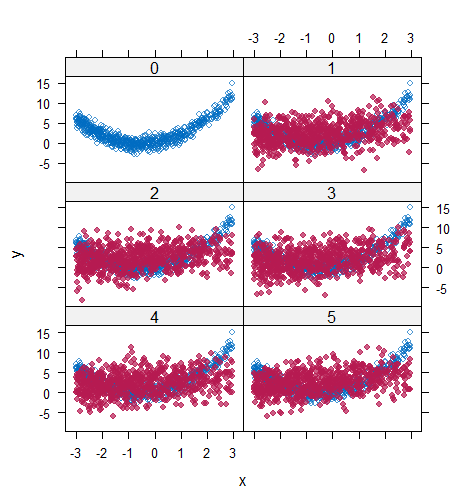
\includegraphics[scale=.5]{plot/6}
			}
		}
	\end{center}
	\caption{Scatterplots and densityplots are generated under 30\% missing cases and MARr missingness mechanism.}
	\label{fig3}
\end{figure}

\begin{figure}[ht!]
	\begin{center}
		\resizebox{\textwidth}{!}{
			\subfigure[quadratic imputation model]{
				\label{boxplot:a}
				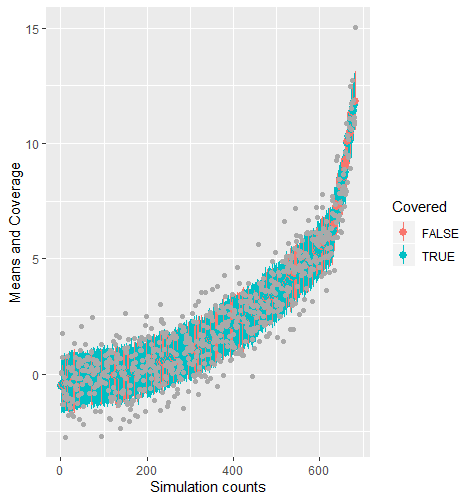
\includegraphics[scale=.5]{plot/7}
			}
			\subfigure[linear imputation model]{
				\label{boxplot:b}
				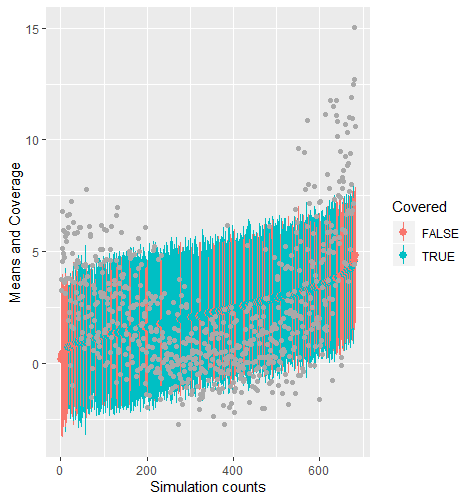
\includegraphics[scale=.5]{plot/8}
			}
		}
	\end{center}
	\caption{Distribution plots are generated under 30\% missing cases and MARr missingness mechanism. The confidence interval is 75\% nominal.}
	\label{fig4}
\end{figure}

\begin{sidewaysfigure}[ht!]
	\begin{center}
		\resizebox{\textwidth}{!}{
			\subfigure[PC]{
				\label{boxplot:a}
				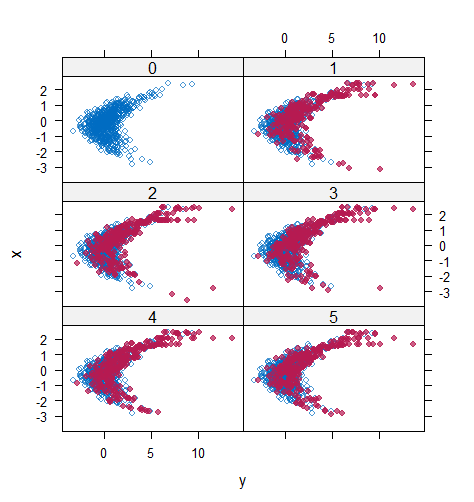
\includegraphics[scale=.5]{plot/scatterpc}
			}
			\subfigure[SMC-FCS]{
				\label{boxplot:b}
				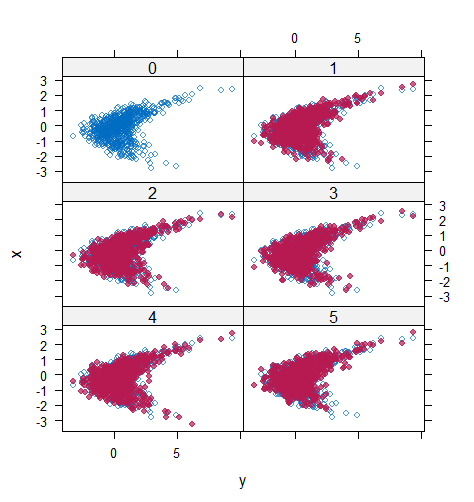
\includegraphics[scale=.5]{plot/scattersmcfcs}
			}
			\subfigure[PMM]{
				\label{boxplot:b}
				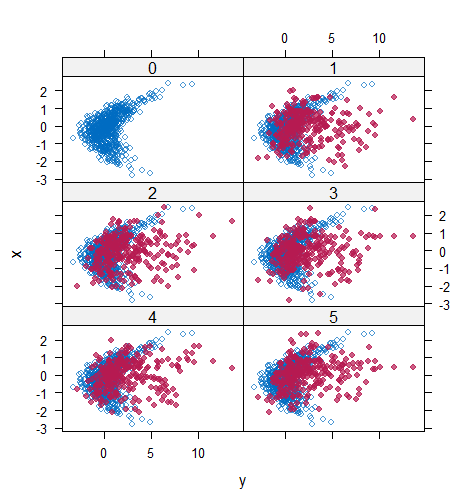
\includegraphics[scale=.5]{plot/scatterpmm}
			}
		}
	\end{center}
	\caption{Scatterplots generated under 30\% missing cases and MARr missingness mechanism.}
	\label{fig5}
\end{sidewaysfigure}
\begin{sidewaysfigure}[ht!]
	\begin{center}
		\resizebox{\textwidth}{!}{
			\subfigure[PC]{
				\label{boxplot:a}
				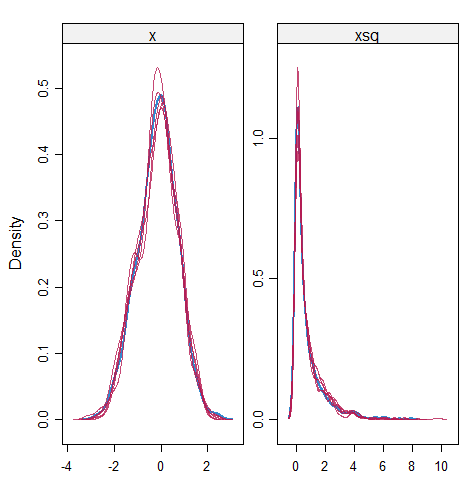
\includegraphics[scale=.5]{plot/densitypc}
			}
			\subfigure[SMC-FCS]{
				\label{boxplot:b}
				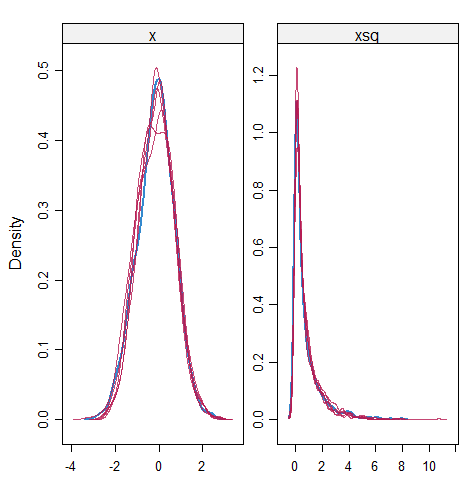
\includegraphics[scale=.5]{plot/densitysmcfcs}
			}
			\subfigure[PMM]{
				\label{boxplot:b}
				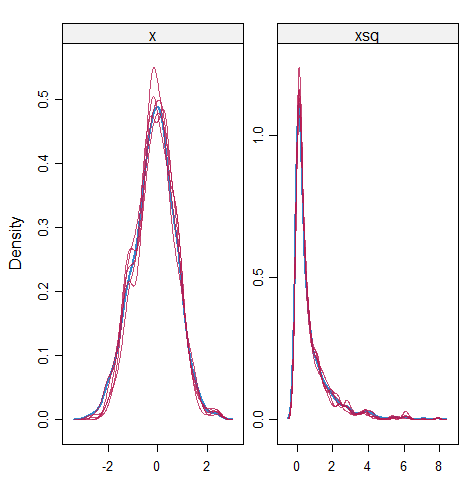
\includegraphics[scale=.5]{plot/densitypmm}
			}
		}
	\end{center}
	\caption{Densityplots generated under 30\% missing cases and MARr missingness mechanism.}
	\label{fig6}
\end{sidewaysfigure}
\begin{sidewaysfigure}[ht!]
	\begin{center}
		\resizebox{\textwidth}{!}{
			\subfigure[PC]{
				\label{boxplot:a}
				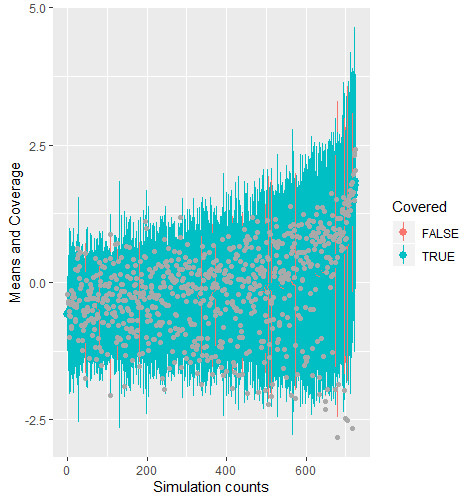
\includegraphics[scale=.5]{plot/distributionpc}
			}
			\subfigure[SMC-FCS]{
				\label{boxplot:b}
				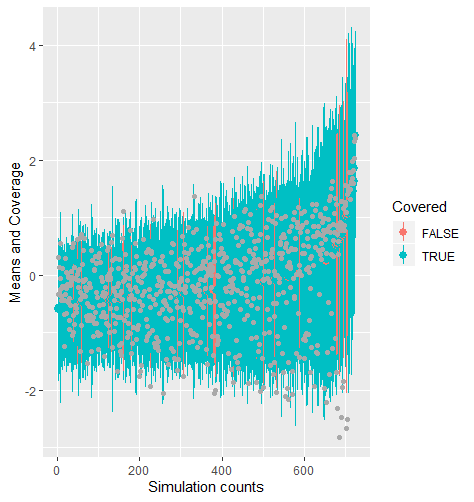
\includegraphics[scale=.5]{plot/distributionsmcfcs}
			}
			\subfigure[PMM]{
				\label{boxplot:b}
				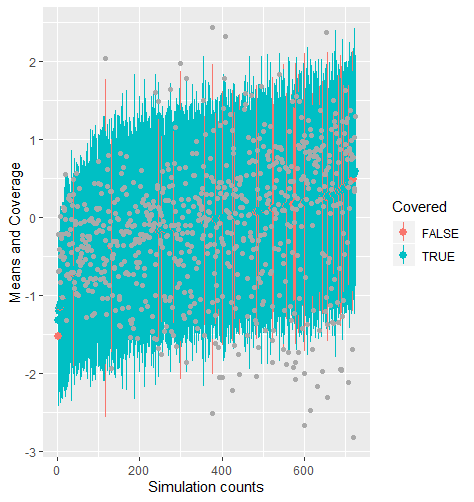
\includegraphics[scale=.5]{plot/distributionpmm}
			}
		}
	\end{center}
	\caption{Distributionplots generated under 30\% missing cases and MARr missingness mechanism. The nominal level is 95\%.}
	\label{fig7}
\end{sidewaysfigure}
\begin{sidewaysfigure}[ht!]
	\begin{center}
		\resizebox{\textwidth}{!}{
			\subfigure[PC]{
				\label{boxplot:a}
				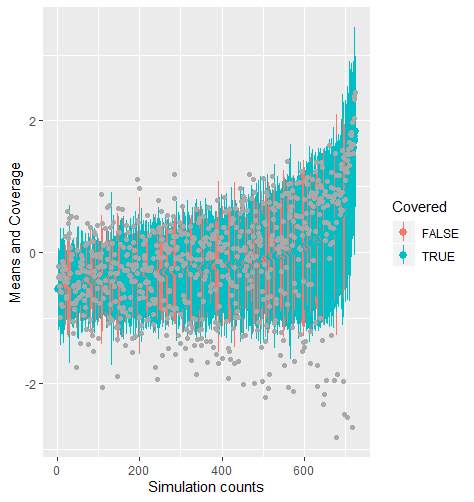
\includegraphics[scale=.5]{plot/distribution75pc}
			}
			\subfigure[SMC-FCS]{
				\label{boxplot:b}
				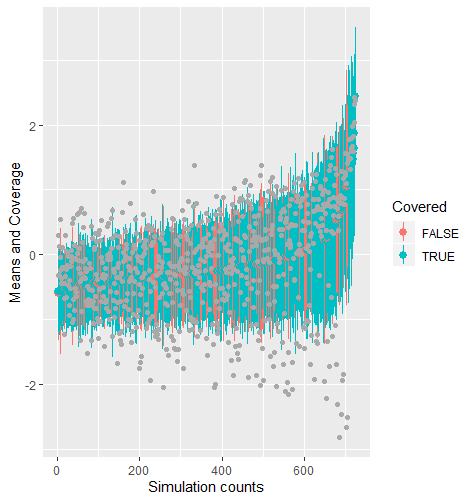
\includegraphics[scale=.5]{plot/distribution75smcfcs}
			}
			\subfigure[PMM]{
				\label{boxplot:b}
				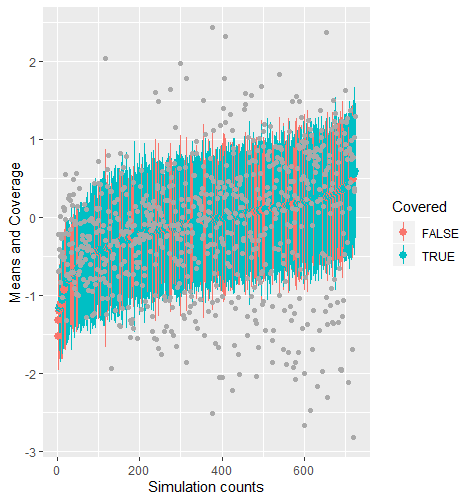
\includegraphics[scale=.5]{plot/distribution75pmm}
			}
		}
	\end{center}
	\caption{Distributionplots generated under 30\% missing cases and MARr missingness mechanism. The nominal level is 75\%.}
	\label{fig8}
\end{sidewaysfigure}

\begin{figure}[ht!]
	\begin{center}
		\resizebox{\textwidth}{!}{
			\subfigure[logistic model based on $X$ and $Z$]{
				\label{boxplot:a}
				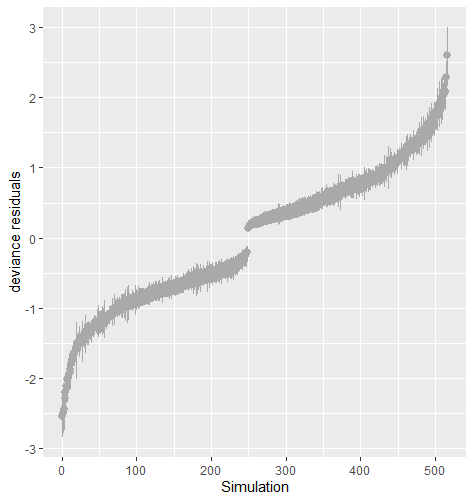
\includegraphics[scale=.5]{plot/deviancewithx}
			}
			\subfigure[logistic model based on $Z$]{
				\label{boxplot:b}
				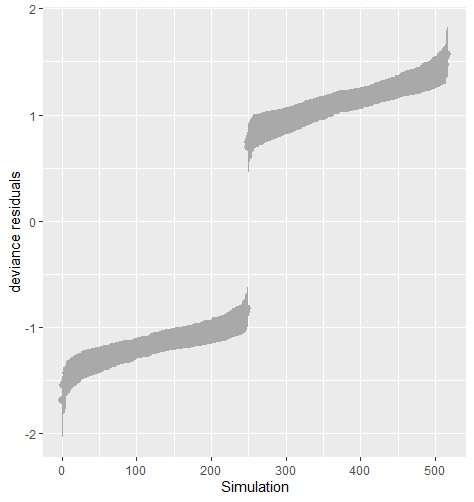
\includegraphics[scale=.5]{plot/deviancewithoutx}
			}
		}
	\end{center}
	\caption{The plot of deviance residuals generated  under two logistic regression imputation models. The percentage of missing is 30\% and the missingness mechanism is MARr.}
	\label{fig9}
\end{figure}
\begin{figure}[ht!]
	\begin{center}
		\resizebox{\textwidth}{!}{
			\subfigure[logistic model based on $X$ and $Z$]{
				\label{boxplot:a}
				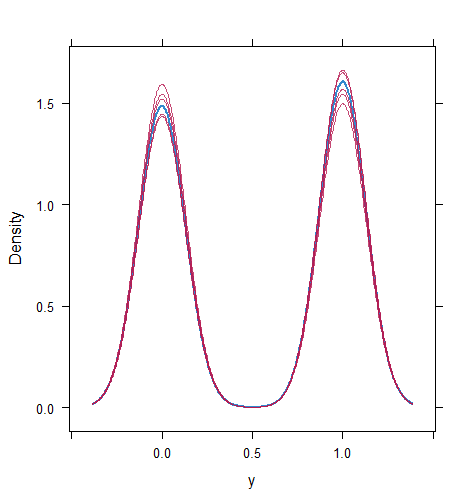
\includegraphics[scale=.5]{plot/densitywithx}
			}
			\subfigure[logistic model based on $Z$]{
				\label{boxplot:b}
				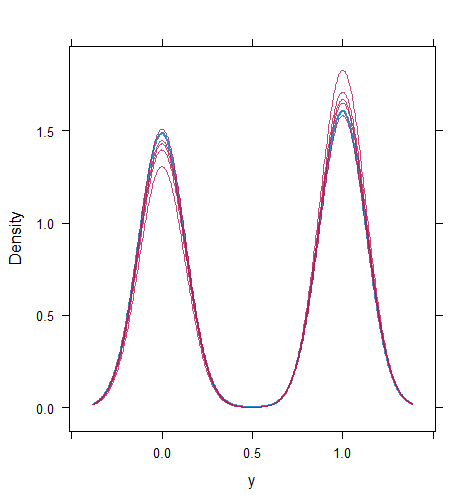
\includegraphics[scale=.5]{plot/densitywithoutx}
			}
		}
	\end{center}
	\caption{The density plots generated under two logistic regression imputation models. The percentage of missing is 30\%, and the missingness mechanism is MARr.}
	\label{fig10}
\end{figure}


\begin{figure}[ht!]
	\begin{center}
		\resizebox{\textwidth}{!}{
			\subfigure[densityplot in case 1]{
				\label{boxplot:a}
				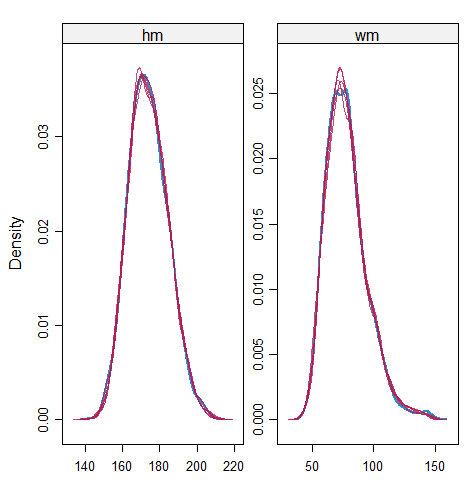
\includegraphics[scale=.5]{plot/densitycase1}
			}
			\subfigure[scatterplot of hm in case 1]{
				\label{boxplot:b}
				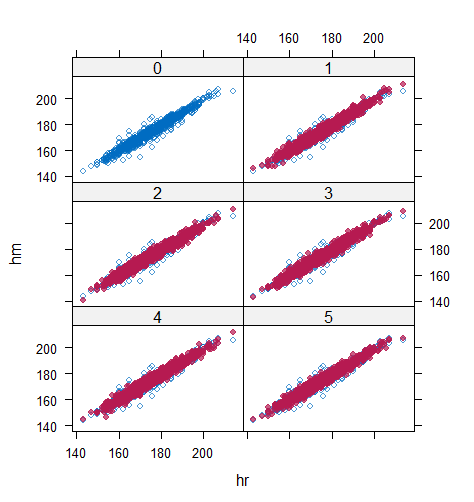
\includegraphics[scale=.5]{plot/scattercase1hm}
			}
		}\\ 	
		\resizebox{\textwidth}{!}{
			\subfigure[scatterplot of wm in case 1]{
				\label{boxplot:c}
				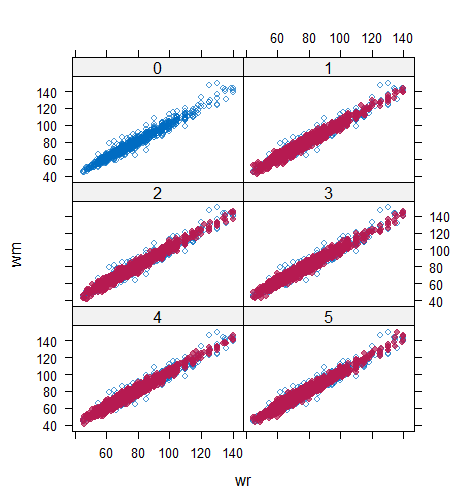
\includegraphics[scale=.5]{plot/scattercase1wm}
			}
			\subfigure[distribution plot of hm in case 1]{
				\label{boxplot:d}
				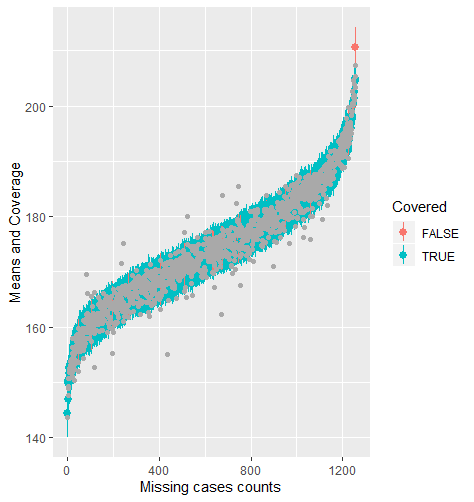
\includegraphics[scale=.5]{plot/distributioncase1hm}
			}
		}
	    \resizebox{\textwidth}{!}{
		\subfigure[distribution plot of wm in case 1]{
			\label{boxplot:e}
			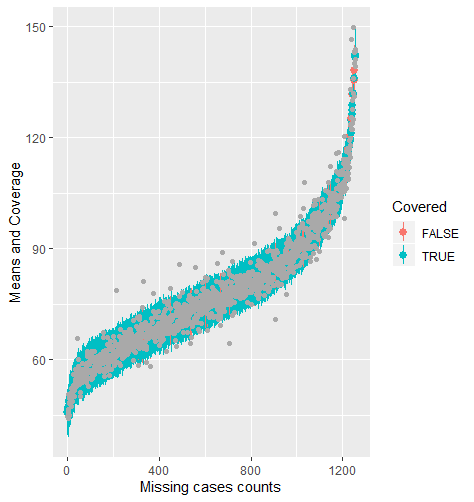
\includegraphics[scale=.5]{plot/distributioncase1wm}
		}
		\subfigure[densityplot in case 2]{
			\label{boxplot:f}
			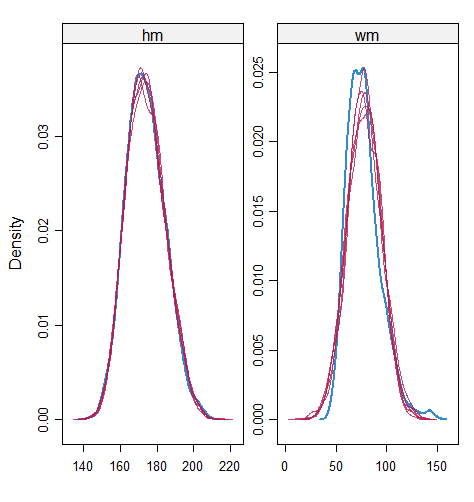
\includegraphics[scale=.5]{plot/densitycase2}
		}
	}
\end{center}
\caption{Graphical analysis of the BMI data}
\label{fig11}
\end{figure}
\begin{figure}[ht!]
	 \begin{center}
         \resizebox{\textwidth}{!}{
         	\subfigure[scatterplot of hm in case 2]{
         		\label{boxplot:a}
         		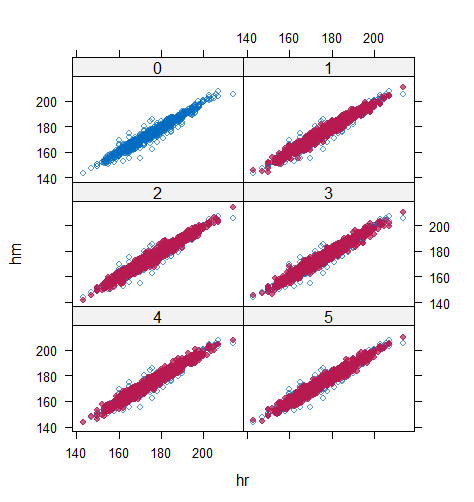
\includegraphics[scale=.5]{plot/scattercase2hm}
         	}
         	\subfigure[scatterplot of wm in case 2]{
         		\label{boxplot:b}
         		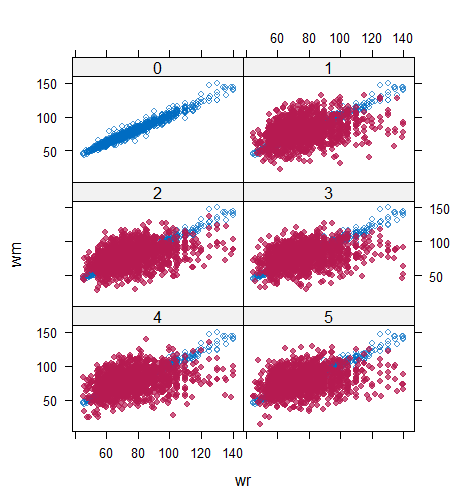
\includegraphics[scale=.5]{plot/scattercase2wm}
         	}
         }\\
         \resizebox{\textwidth}{!}{
         	\subfigure[distribution plot of hm in case 2]{
         		\label{boxplot:c}
         		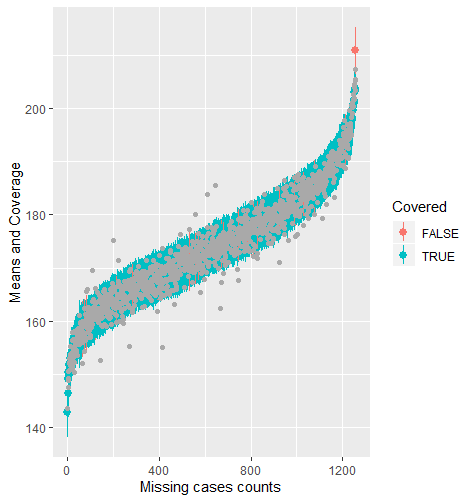
\includegraphics[scale=.5]{plot/distributioncase2hm}
         	}
         	\subfigure[distribution plot of wm in case 2]{
         		\label{boxplot:d}
         		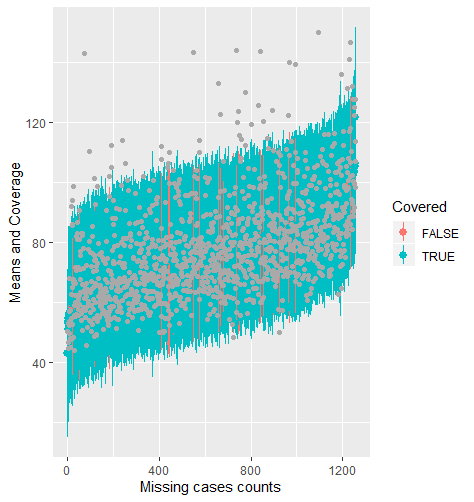
\includegraphics[scale=.5]{plot/distributioncase2wm}
         	}
         }\\
        \resizebox{\textwidth}{!}{
        	\subfigure[densityplot in case 3]{
        		\label{boxplot:e}
        		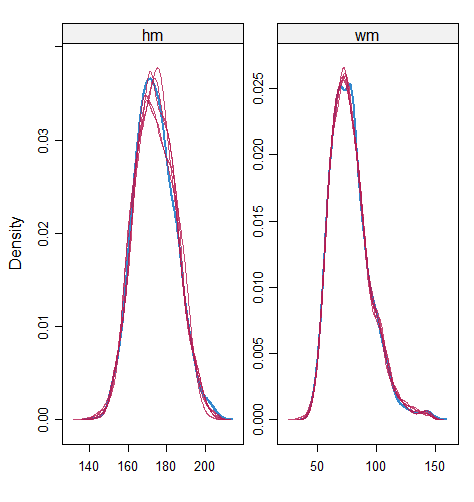
\includegraphics[scale=.5]{plot/densitycase3}
        	}
        	\subfigure[scatterplot of hm in case 3]{
        		\label{boxplot:f}
        		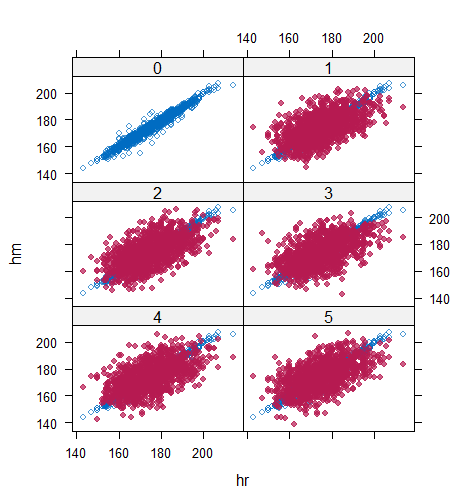
\includegraphics[scale=.5]{plot/scattercase3hm}
        	}
        }
    
    \end{center}
\caption{Graphical analysis of the BMI data}
\label{fig12}
\end{figure}

\begin{figure}[ht!]
	\begin{center}	
        \resizebox{\textwidth}{!}{
        	\subfigure[scatterplot of wm in case 3]{
        		\label{boxplot:a}
        		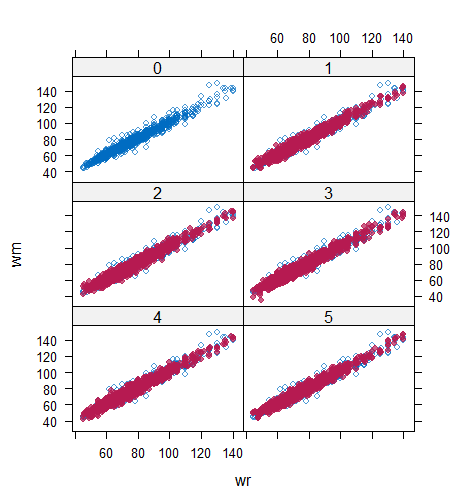
\includegraphics[scale=.5]{plot/scattercase3wm}
        	}
        	\subfigure[distribution plot of hm in case 3]{
        		\label{boxplot:b}
        		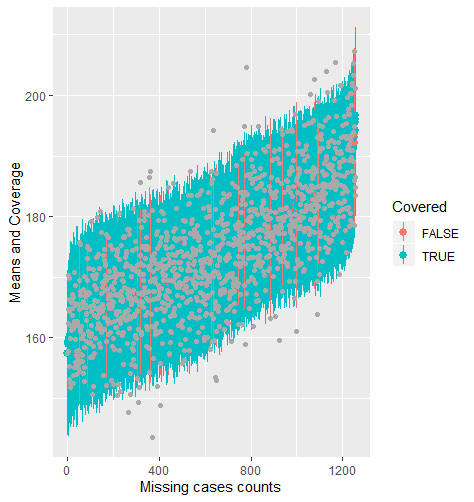
\includegraphics[scale=.5]{plot/distributioncase3hm}
        	}
        }
        \resizebox{\textwidth}{!}{
        	\subfigure[distribution plot of wm in case 3]{
        		\label{boxplot:c}
        		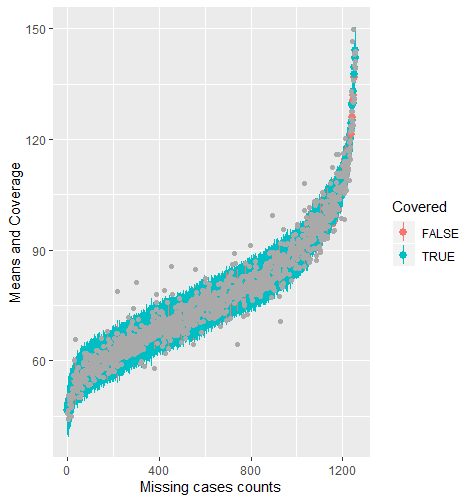
\includegraphics[scale=.5]{plot/distributioncase3wm}
        	}
        	\subfigure[densityplot in case 4]{
        		\label{boxplot:d}
        		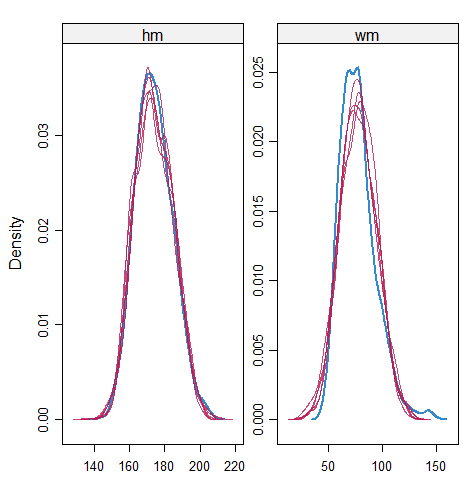
\includegraphics[scale=.5]{plot/densitycase4}
        	}
        }\\ 
        \resizebox{\textwidth}{!}{
        	\subfigure[scatterplot of hm in case 4]{
        		\label{boxplot:e}
        		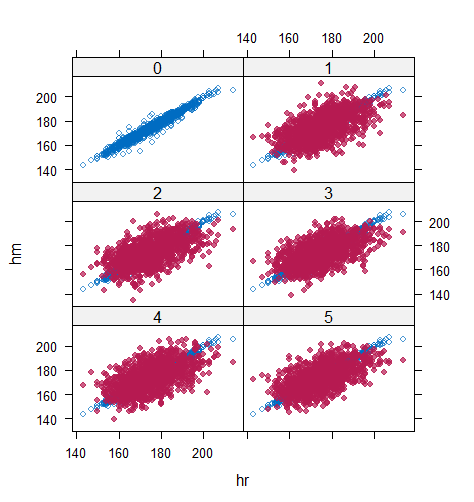
\includegraphics[scale=.5]{plot/scattercase4hm}
        	}
        	\subfigure[scatterplot of wm in case 4]{
        		\label{boxplot:f}
        		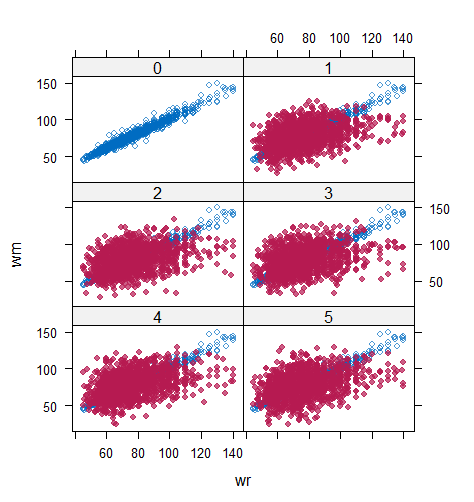
\includegraphics[scale=.5]{plot/scattercase4wm}
        	}
        }
    \end{center}
\caption{Graphical analysis of the BMI data}
\label{fig13}
\end{figure}
\begin{figure}[ht!]
	\begin{center}
        \resizebox{\textwidth}{!}{
        	\subfigure[distribution plot of hm in case 4]{
        		\label{boxplot:s}
        		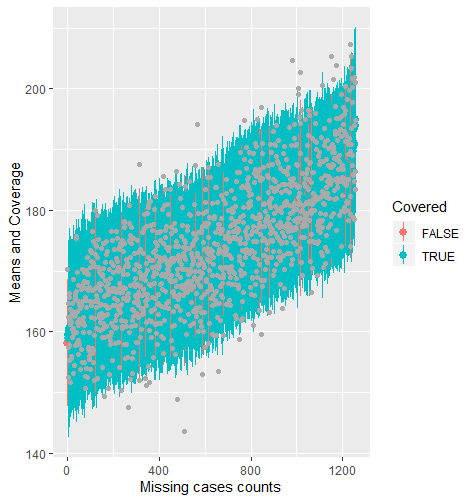
\includegraphics[scale=.5]{plot/distributioncase4hm}
        	}
        	\subfigure[distribution plot of wm in case 4]{
        		\label{boxplot:t}
        		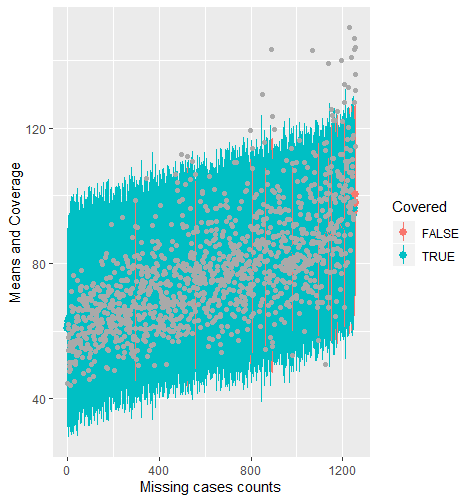
\includegraphics[scale=.5]{plot/distributioncase4wm}
        	}
        }
	\end{center}
\caption{Graphical analysis of the BMI data}
\label{fig14}
\end{figure}


\end{document}